%\chapter{Time- and power-stability of the X-ray tube}\label{chap:tps}
\chapter[Time- Power-Stability]{Time- and power-stability of the X-ray tube}\label{chap:tps}
The following chapter contains the characterization of the time- and power stability properties of the source used at this setup. This qualities are elemental, getting a feeling about the performance of the source. For example a fluctuation in the radiation-output during a measurement can destroy the whole outcome, because e.g. a correction with a flatfield does not properly cancel out the influence of the source-spectrum during the measurement.   
\section{Time-stability}\label{sec:time}
First of all the time performance of the source is examined in a more detailed way, to have a first impression how stable is the performance of source-output. Therefore a fist measurement of the influence of the exposure time onto the detector response is done, which is usually assumed to be linear for a integrating detector. Knowing this dependency, it is possible to compare images with different exposure-time, but the same X-ray energy and input-power. For example one image is taken with 5 seconds exposure-time and the other with 10 seconds, one can compare them by simple multiplication or division of the intensity in one image with the difference time-factor of the two images, for this case also by a factor of 2. This knowledge is very helpful, because especially in material research the dose is not the limiting factor and one can spare a lot of measurement time. \textcolor{red}{weiß nicht ob das so gut als beispiel passt} The dependency of the detector used for this thesis is shown in Fig: \ref{exposetime}. At the left side the dependency is shown in a plot with linear scaled axes. For better insight onto the variations the same data are plotted as well on the right side on double logarithmic scaled axes. Obviously is the behaviour on the left side as well as on the right side really linear, which is very positive for the further characterization. Furthermore show these plots already a first advice onto the stability of the source-output, because fluctuations within the source intensity, would destroy the linear behaviour.
\begin{figure}[h]
	\begin{center}
		\includegraphics[width = 14.7cm,keepaspectratio = true]{exposetimecombi}
	\end{center}
	\caption[Dependency of the detector response onto the exposure time]{\textit{Dependency between the detector response onto a steady source output intensity during different exposure times. The left plot shows the measured data points and the corresponding linear regression on linearly scaled axes. The right plot illustrates the same data and their regression, but on a double logarithmic scale. The big benefit of this plot is, that variations within the recorded intensity have much more influence on the logarithmic scale than on a linear one.}}
	\label{exposetime}
\end{figure}

\paragraph{Long- time stability}
As a next step the long time behaviour of the source is examined in more detail. This property is of big importance e.g for tomographic measurements, because they are very time extensive. The main problem of a variation of the source intensity for this case is, that due to this artefacts are induced in the latter tomographic reconstruction. If the intensity e.g. drops down during the measurement the first projections have better statistics and are brighter, than the projections at the end. Therefore usually flat-field images are taken in between the respective projection blocks. A flat-field image is a picture without any sample, so just the pure source-intensity distribution is recorded. The projection images are then afterwards corrected by division with theses flat-fields to avoid the influence of the intensity drop. As one can imagine, the frequency taking such flat-fields is again a trade off between time effort and precision. So for the case that the time behaviour of the source is well-known one can e.g. adjust the frequency of the flat-fields, but regardless of the respective measurement technique the stable the source the better. For the determination of the time-stability of the source used for this thesis a phase tomography data-set recorded of Friedrich Prade is taken. The complete measurement time was around two days and within these two days every 20 minutes a block of stepped flat-fields is taken to correct the projection images. With the stepping routine described in \ref{subsec:stepp} one can retrieve the corresponding mean intensity and the visibility, whereby the mean intensity is just the parameter $a_{0}$ within a region of the image without any gratings. The Values for this two parameters are depicted in Fig:\ref{2daysstabi}. The left side shows the mean intensity averaged over three sections of the images without gratings, and the right side shows the mean visibility without any sample.       
\begin{figure}[t]
	\begin{center}
		\includegraphics[width = 14.7cm,keepaspectratio = true]{2daystability}
	\end{center}
	\caption[Time-stability of the source during two days]{\textit{Time stability of the source in between two days. The left side shows the fluctuation of the mean intensity during the measurement, the right side shows the corresponding visibility. The data points are extracted from the flat-fields taken between two projection blocks. The variation over the time is in both cases very small. The mean intensity varies $\approx1$ \% which is very low and also the visibility varies just about $\approx 4.5$ \% compared to the start value, respectively.}}
	\label{2daysstabi}
\end{figure}
The variation of the intensity varies with respect to the start value around $\approx 1$ \% which is on this time scale very low and with disregarding the spike at about 2.5 hours the variation is even lower of $\approx 7$ \permil. The change of the visibility during the measurement time of $\approx 4.5$ \% is a bit higher with respect to the start value of $21,35$ \% but still in a good region. 
\section{Power-stability}\label{sec:power}
After the determination of the time-stability of the source also the power-stability is an important property, which is worth to be characterized. The procedure is a very easy one. In this case the energy and the exposure time is fixed to a distinct value for this case the energy of the electrons is set to 60 keV and the exposure time is for the first measurement set to 10 and for the second to 5 seconds, respectively. With the linear behaviour discovered in the latter section, the second data are multiplied by a factor of two for a better comparison. Tuning the power of the source by a fixed energy results in a change of the emission current of the filament, which results in more or less emitted electrons producing X-rays. The behaviour of the function  $P \text{[W]} =U \cdot I$  with a fixed $U$ and the constant electron charge $e$, should result in a more or less linear function, but the main interest of this measurement lies on the resulting intensity of the X-rays instead of directly measuring the applied current. The plot in Fig:\ref{powerdep} shows therefore the intensity averaged over the centre of the recorded image versus the power. As mentioned above, there are two measurements with a time delay of about half a year, double checking the dependency and especially the drop of the intensity in all four curves at about $25-40$ Watt. In each measurement, the mean intensity is measured one time with the usual gratings inside the beam and one time without them. Hence, also the pure attenuation due to absorption of the grating materials is explored. As one can see the two curves with gratings lie over the whole power range always close together, whereupon the both without gratings differ more and more during the measurement. One possible explanation for this is, that due to the confined lifetime of the filament one measurement took place at the end of such a period, so there were less X-ray photons produced. Another explanation is a small change in the source spectrum, because the loss of intensity is just distinguishable in the case without gratings. This means that the spectrum for the latter measurement was possibly shifted to slightly lower photon energies, because lower photons contribute less to the intensity than high energy. This is also in accordance to the curves with gratings, because photons with lower energy are almost completely absorbed in the grating material and have thus for both measurements no contribution to the intensity within the image. As one can see is the drop at $25-40$ Watt no measurement error, but rather an intrinsic source property. 
\begin{figure}%[h]
	\begin{center}
		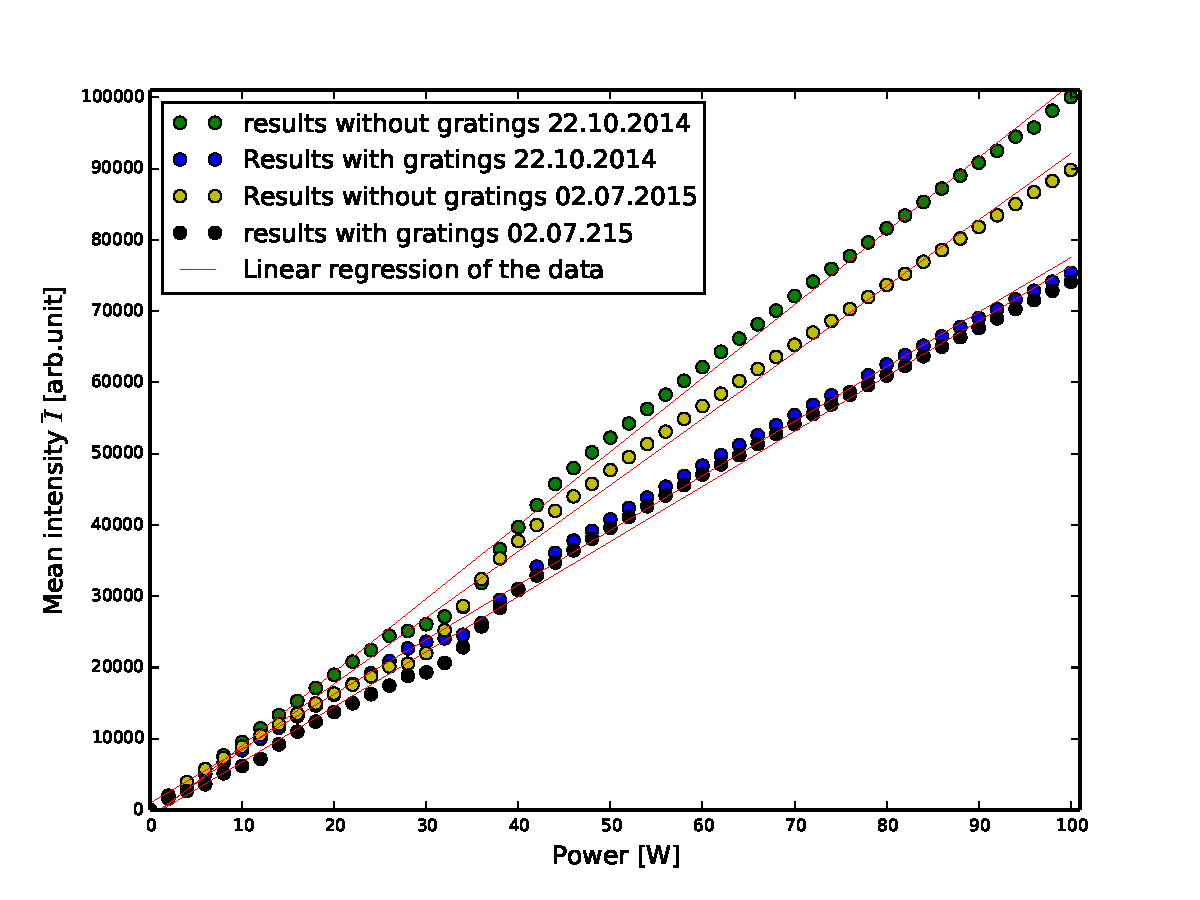
\includegraphics[width = 14.7cm,keepaspectratio = true]{power}
	\end{center}
	\caption[Power-stability of the source with fixed energy to 60 kV]{\textit{Behaviour of the power-stability of the source for a fixed energy at 60 kV. The plot shows four different data sets for two different dates. The Two sets marked with blue and black dots show the source behaviour with gratings in the beam, the two with yellow and green dots without anything inside the beam. }}
	\label{powerdep}
\end{figure}
The explanation lies within the electron optic of the source. As mentioned in section \ref{subsec:dimstruc} and shown in Fig:\ref{sourcerotfoc} this optic focusses the electron beam down to a very small area. But this is just possible for a distinct power range, because otherwise would the target be severely damaged by the deposition of to much heat on a to small area. Hence, the focus coils have to open up. Unfortunately this is not happening smoothly but rather at a distinct power for this case at $25$ Watt. After this the impact area on the target increases rapidly until a distinct point. A side-effect of this is a loss of intensity, because more electrons just deposit their energy in terms of heat within the target material. \textcolor{red}{ist glaub ich nicht so ganz richtig}

\paragraph{Conclusion}
In summary on can say, that the performance of the source is for both cases in time- as well in power-stability in a good position. Of course is the variation in time and power influenced by several internal and external factors, but these results give a good rule of thumb improving the future measurements. Maybe they can even explain some artefacts in the recorded images or on can improve with this the image quality and also shorten the expenditure of time. For example in the flat-field case it is senseless to take a \gls{flat} after one or two projections if the source is stable for a longer time period. 
\textcolor{red}{hier muss noch mehr hin einfach alles nochmal zusammenfassen? }   
